\chapter{Results and Visualizations}
The previous chapters described the warehouse, the models, the mined rules, and the segments. This chapter shows how those results are delivered to a jury or a review analyst. All results are presented through one eight-page Streamlit application rather than a set of static reports.

\section{Dashboard Architecture}
The dashboard is an eight-page Streamlit app. In the reported deployment it reads the six modelled MART tables directly from Snowflake; this is selected by setting the environment variable \texttt{DATA\_SOURCE=snowflake}. Saved artifacts in the \texttt{artifacts} directory supply the model pipelines, scores, rule sets, and cluster labels. The app never retrains a model on page load, so opening a page reproduces exactly the numbers reported in this document.

Every chart is built with Altair, which gives hover tooltips, zoom, and pan on all plots. The schema drawing on the data model card uses Graphviz. The layout follows the same colour palette as the figures in this report: magenta for the primary series, teal for the secondary series, and amber for accents.

\section{Executive Overview}
\begin{figure}[H]
    \centering
    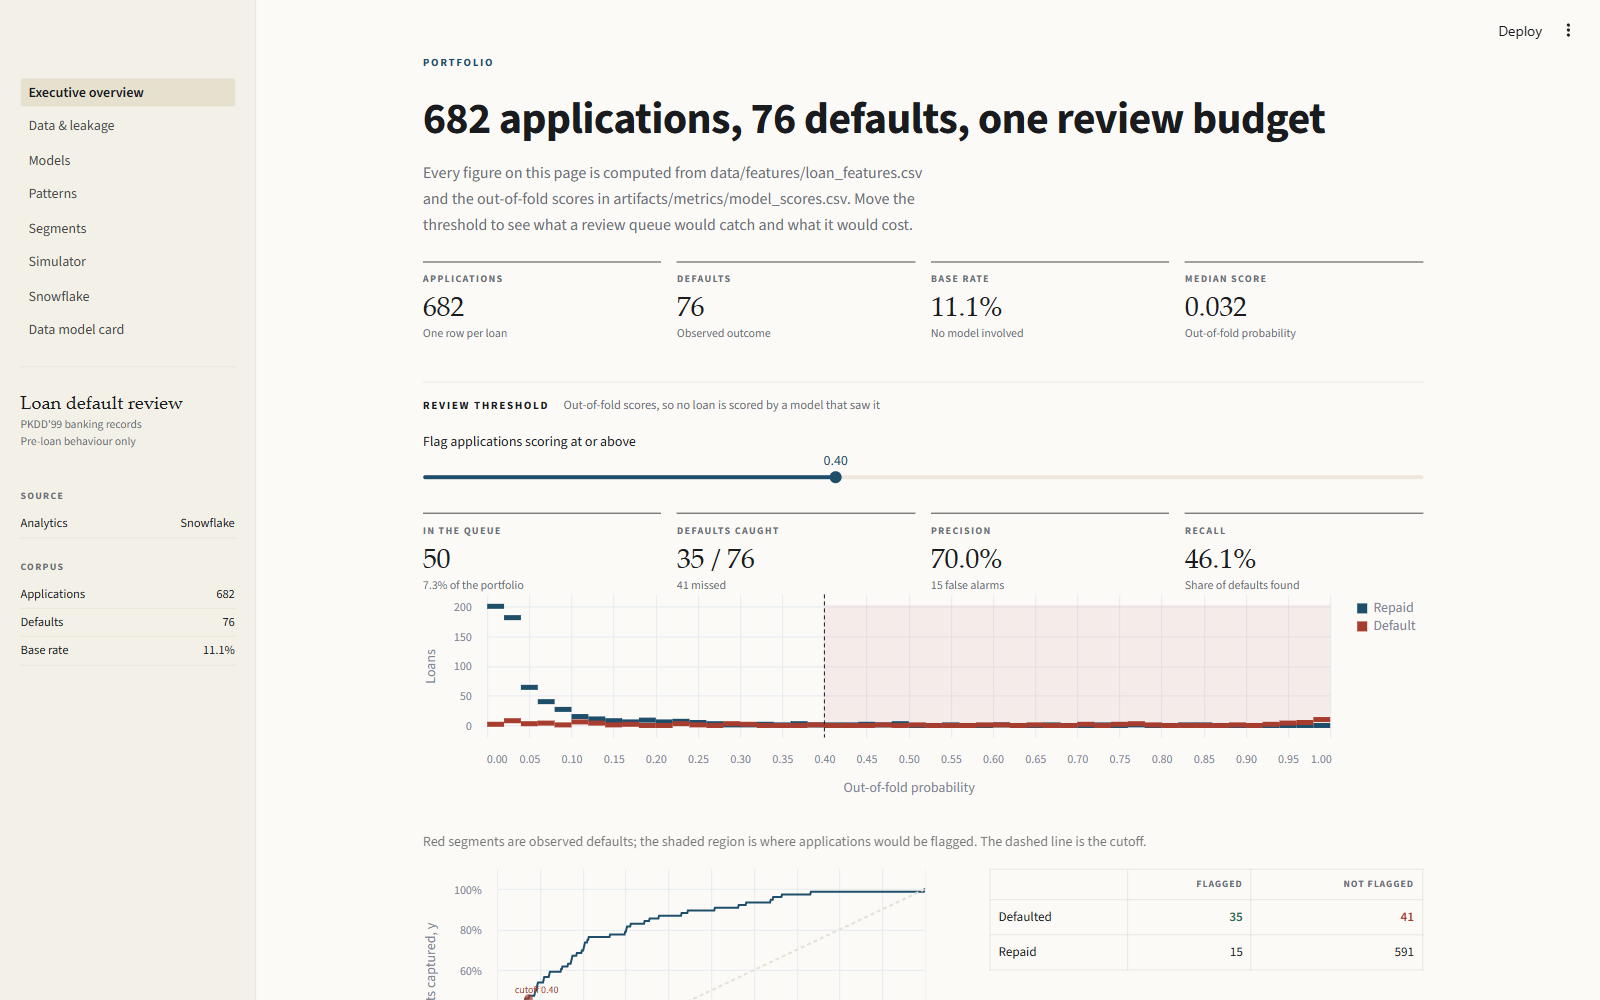
\includegraphics[width=0.92\textwidth]{figures/13_dashboard_executive.png}
    \caption{Executive overview page of the Streamlit dashboard}
    \label{fig:dashboard_executive}
\end{figure}

The executive page is the landing view. A cutoff slider drives the whole page: moving it recomputes the confusion matrix, the exposure figure, and the operating-point metrics from the saved scores. A stacked score histogram shows how defaults and non-defaults distribute across the score range, and a cumulative gains curve shows what share of defaults is captured by reviewing the top-ranked share of the portfolio. A precision/recall trade-off is drawn from a 5\% to 90\% cutoff, and quintile default rates are plotted against the 11.14\% base rate so the lift of ranking is visible at a glance. A segment scatter places loans by their behavioural position, and the selected model's confusion matrix is shown at the current cutoff.

\section{Data and Leakage Page}
\begin{figure}[H]
    \centering
    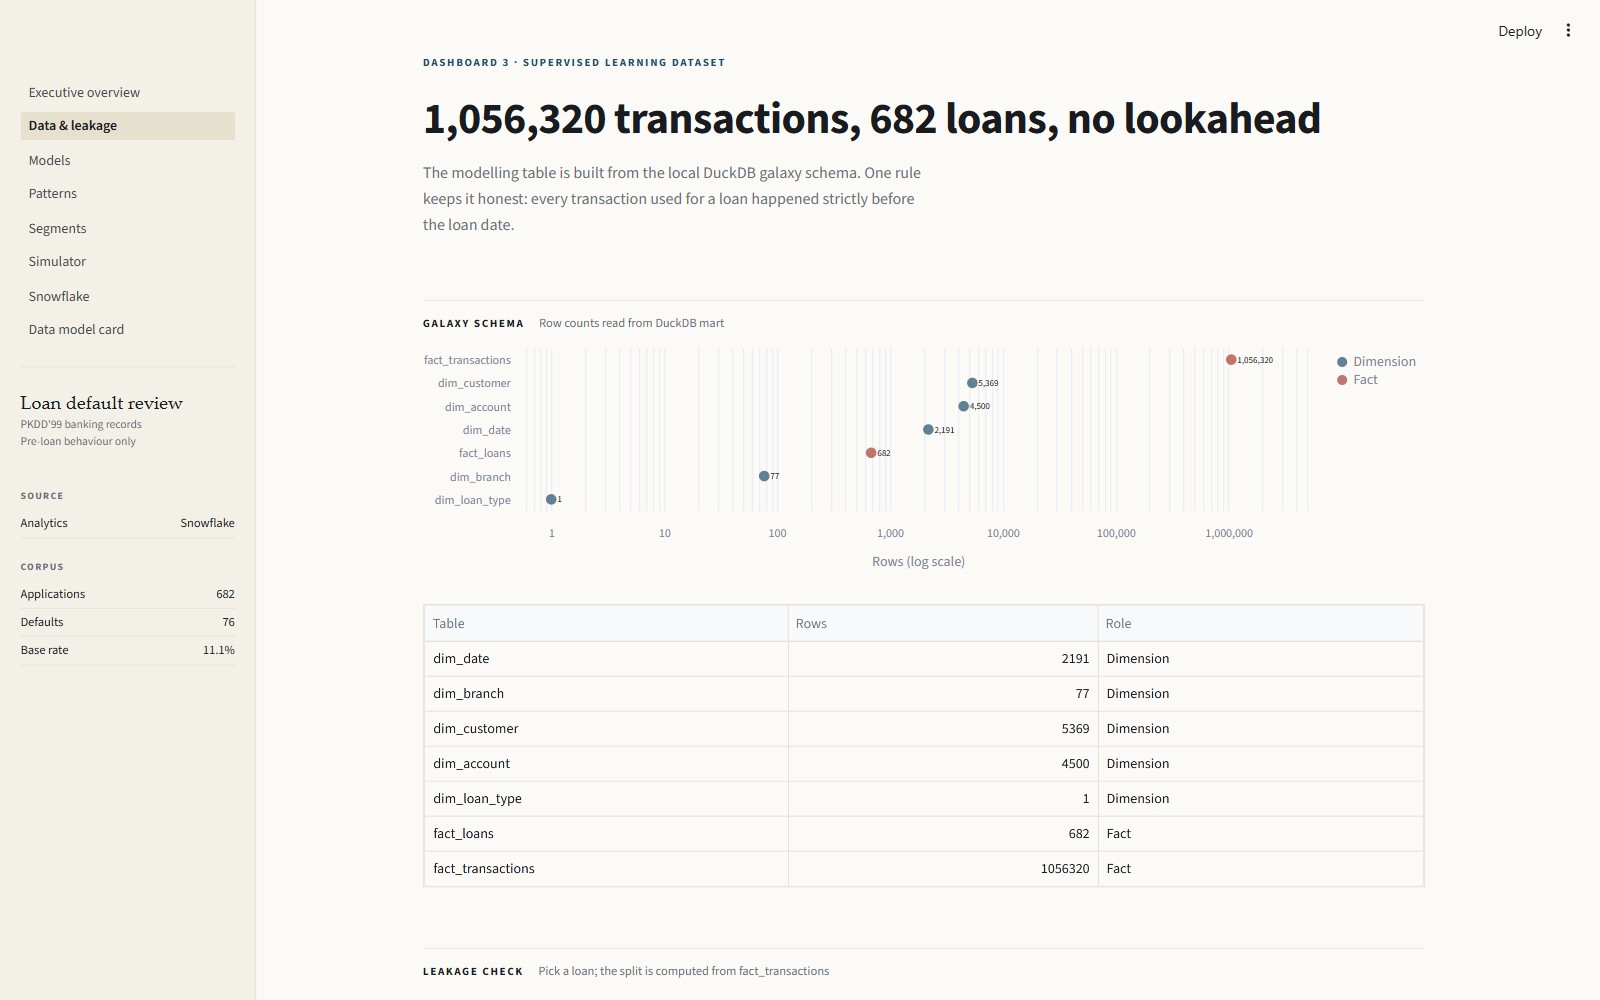
\includegraphics[width=0.92\textwidth]{figures/16_dashboard_data_leakage.png}
    \caption{Data and leakage page of the Streamlit dashboard}
    \label{fig:dashboard_leakage}
\end{figure}

This page is the evidence for the dataset design in Chapter~6. A dot plot shows the row counts of the galaxy-schema tables, so the gap between 682 loans and 1,056,320 transactions is explicit. Per-loan bars show how many transactions were used and how many were excluded by the pre-loan rule; the excluded count is what would have leaked the future. Feature provenance lists each of the 18 modelling features and the table or calculation it comes from, and a set of quality checks reports null counts, duplicate keys, and the post-loan row count of zero.

\section{Models Page}
\begin{figure}[H]
    \centering
    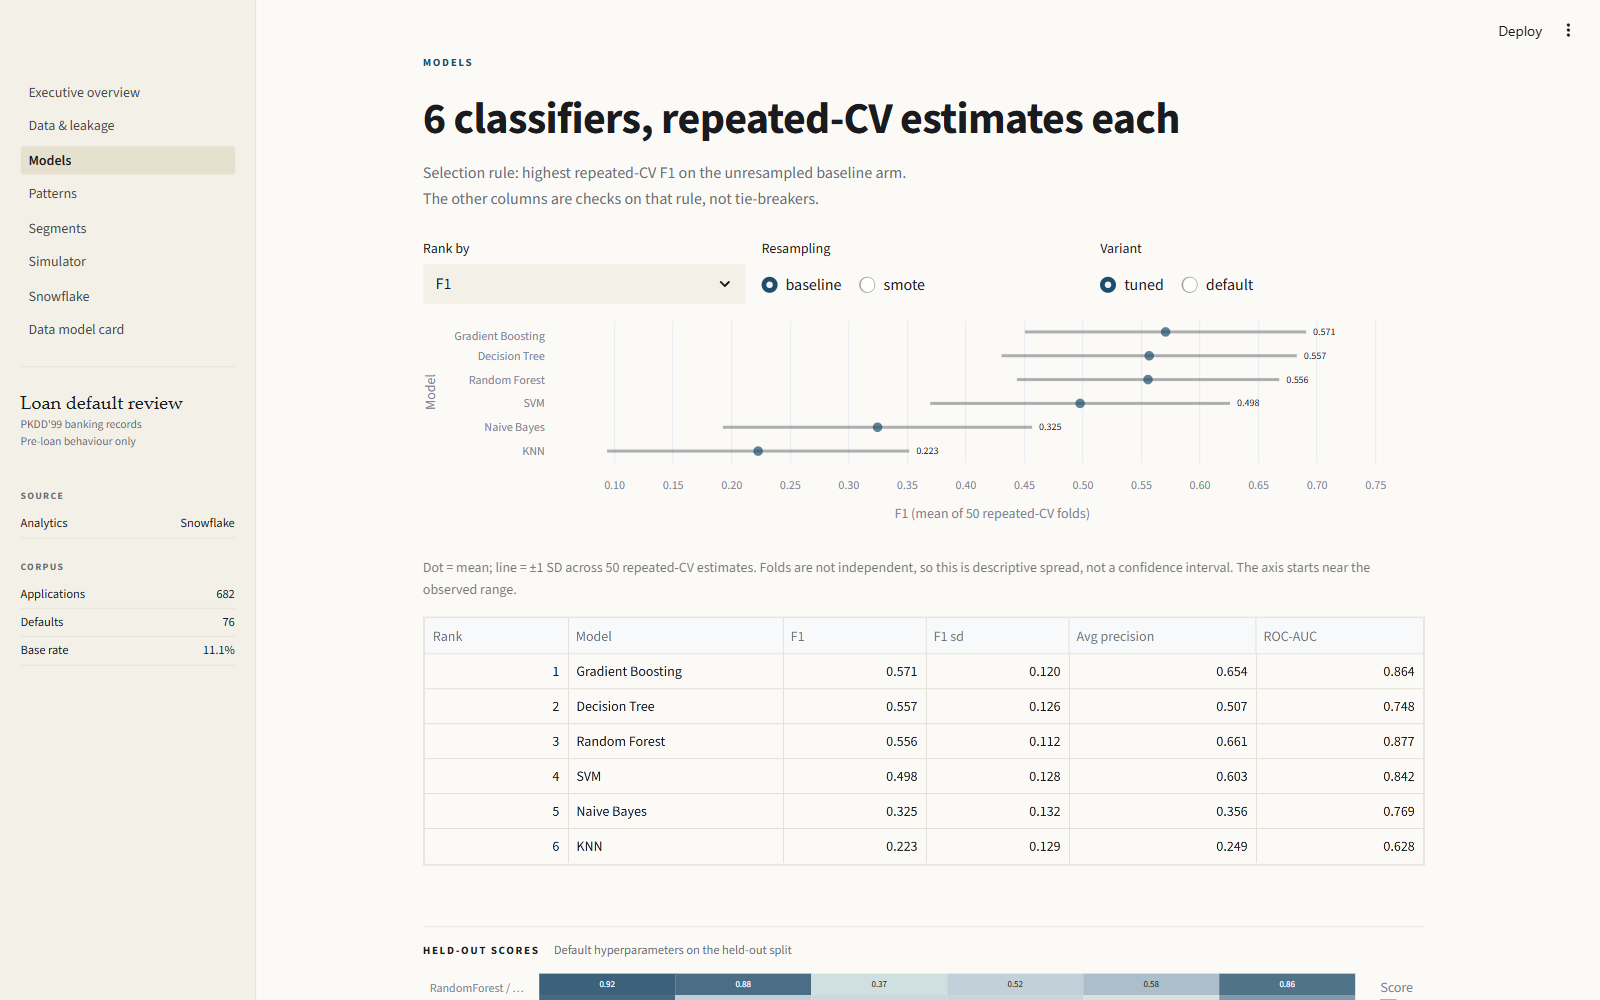
\includegraphics[width=0.92\textwidth]{figures/14_dashboard_models.png}
    \caption{Models page of the Streamlit dashboard}
    \label{fig:dashboard_models}
\end{figure}

The models page consolidates Chapter~8. A metric-aware dot plot shows the repeated-CV mean and one standard deviation for each of the 24 configurations, with a ranking table beside it. A held-out metric heatmap compares F1, average precision, and ROC-AUC across the six classifiers, and ROC and precision/recall curves are drawn for the leading models. A confusion matrix is shown at the default cutoff, tuning results quantify the gain from parameter search, and a challenger dumbbell chart compares the selected tuned Gradient Boosting model with the other algorithms. The chart makes the tied-leading result clear: the tuned Gradient Boosting model leads on F1, while Random Forest leads slightly on average precision and ROC-AUC.

\section{Patterns Page}
\begin{figure}[H]
    \centering
    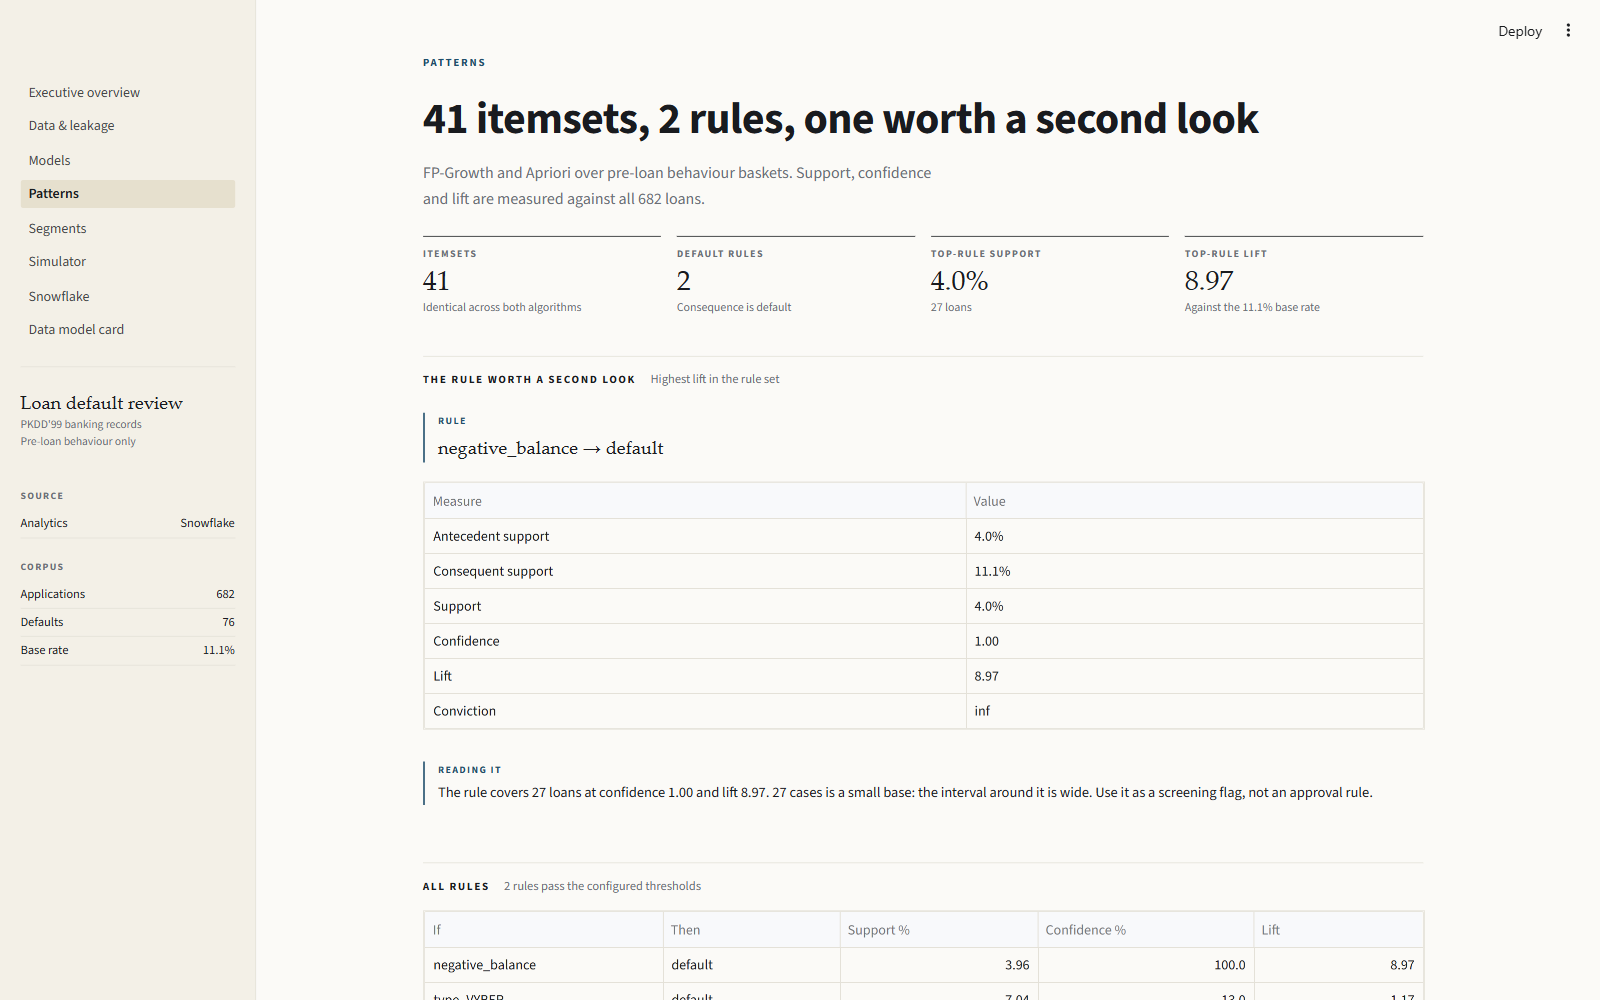
\includegraphics[width=0.92\textwidth]{figures/15_dashboard_patterns.png}
    \caption{Patterns page of the Streamlit dashboard}
    \label{fig:dashboard_patterns}
\end{figure}

The patterns page presents the association rules and the classifier-based rule list. Default rules are ranked by lift, with support and confidence shown beside them. Coverage bars for the classification-based rule set show how many defaults each rule covers, so a high-precision but low-recall rule is not mistaken for a useful screen. Itemset support bars let the jury compare Apriori and FP-Growth on the same baskets; both algorithms return 41 itemsets at a minimum support of 0.03 and a maximum length of three.

\section{Segments Page}
\begin{figure}[H]
    \centering
    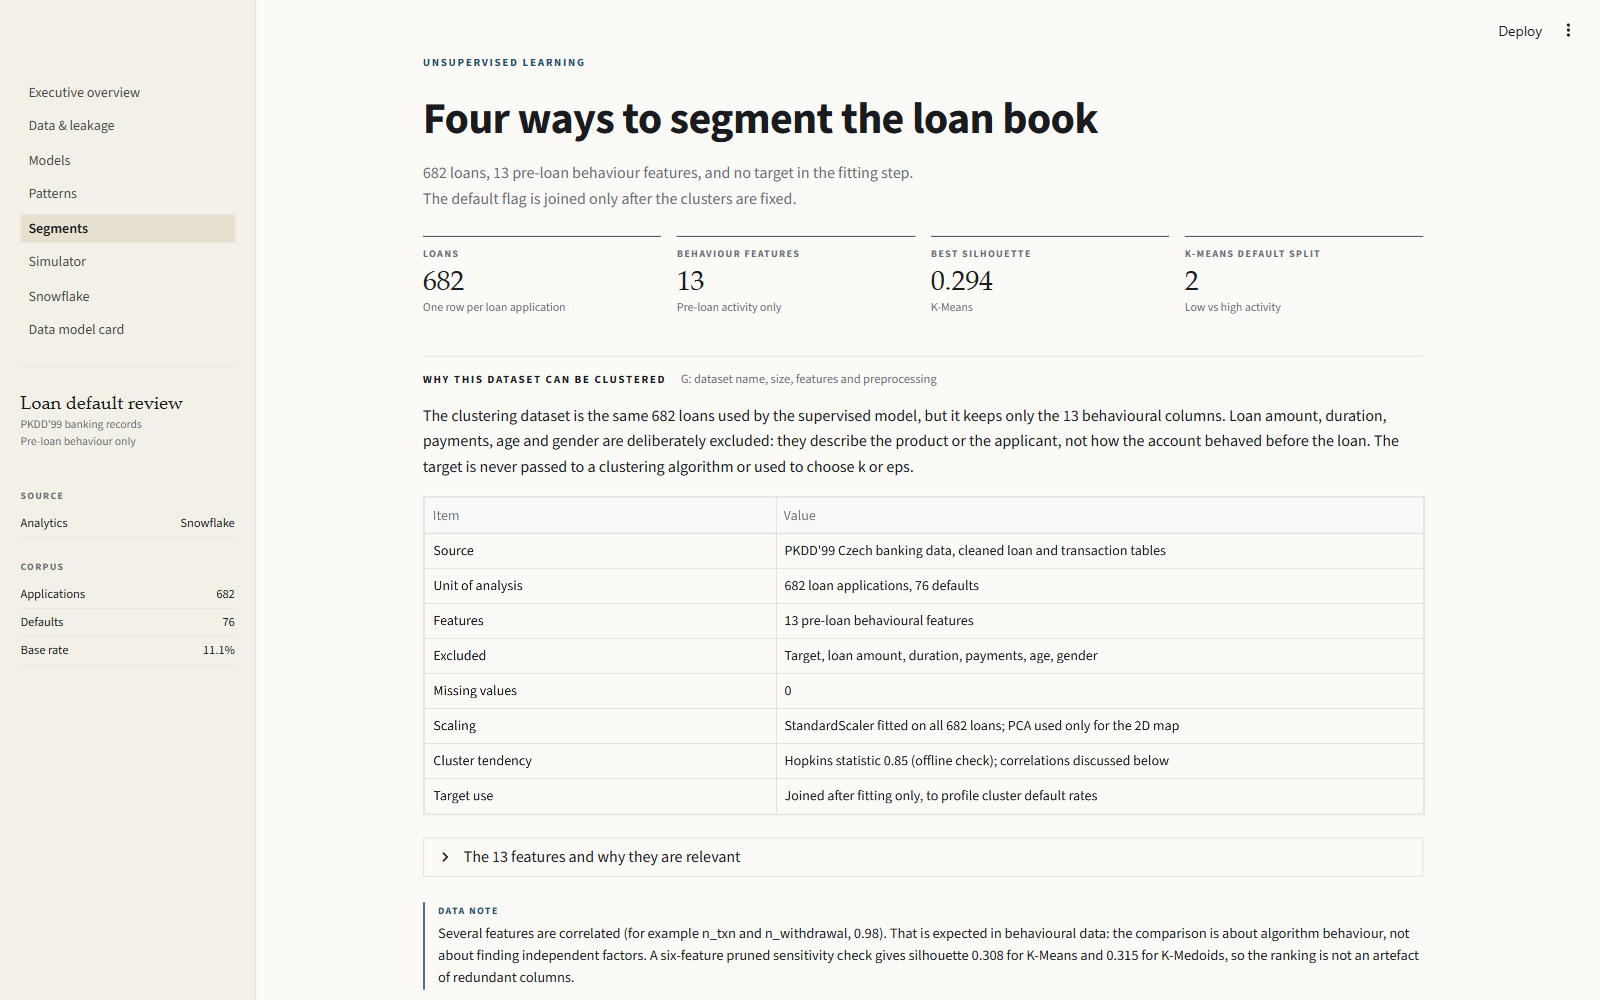
\includegraphics[width=0.92\textwidth]{figures/26_dashboard_segments.png}
    \caption{Segments page of the Streamlit dashboard}
    \label{fig:dashboard_segments}
\end{figure}

The segments page carries the unsupervised results of Chapter~9. A dataset card records that the clustering input is the 13 pre-loan behavioural features with no target. The four-algorithm comparison table is shown with its internal metrics and stability values, and charts compare those metrics visually. PCA maps display the four solutions in two dimensions, cluster profiles describe activity and balance behaviour, and a default-rate chart joins the target back for description only. The page ends with the K-Means verdict and a note that the labels are descriptive, not causal.

\section{Snowflake Deployment Page}

This page is the live counterpart of Chapter~4 and is shown in Figure~\ref{fig:snowflake_page}. It shows the RAW/MART schema split and the 20 expected objects (18 tables plus two views) with their row counts. In Snowflake mode it reads live counts and view samples and displays the verification SQL alongside them. The loader routes raw extracts into RAW and the star schema plus analytics tables into MART, truncating each target before writing so that a rerun is idempotent. This page is what a jury can open to confirm that the deployment is real rather than a diagram.

\section{Simulator Page}
\begin{figure}[H]
    \centering
    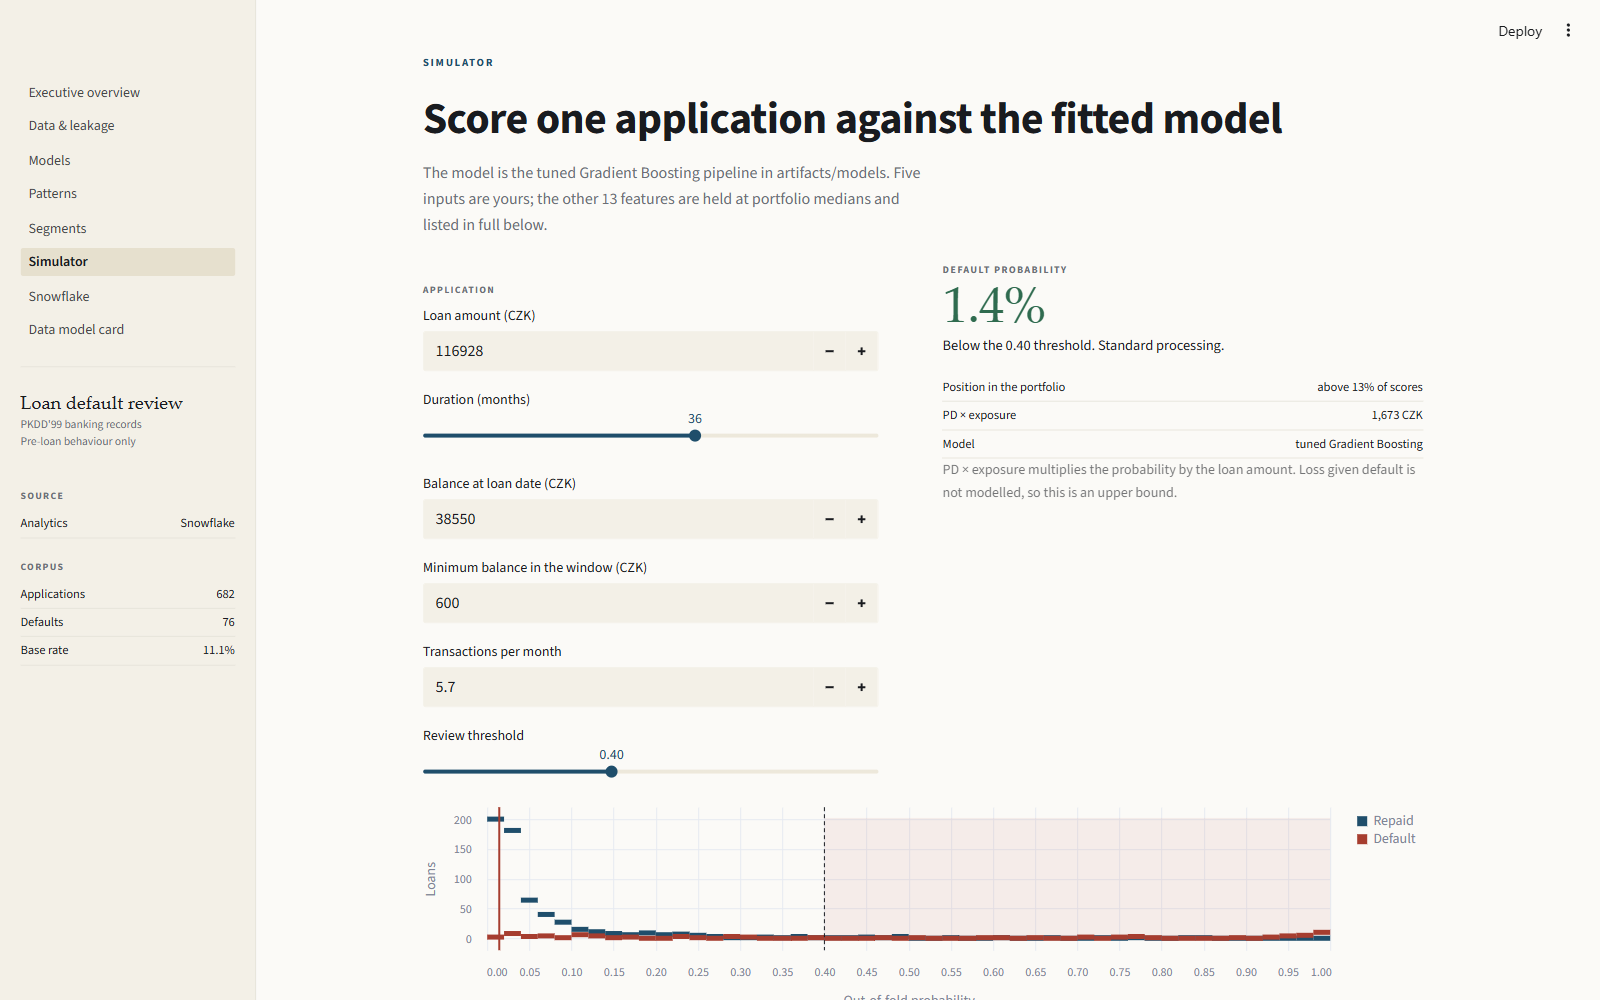
\includegraphics[width=0.92\textwidth]{figures/17_dashboard_simulator.png}
    \caption{Simulator page of the Streamlit dashboard}
    \label{fig:dashboard_simulator}
\end{figure}

The simulator scores a single application with the saved tuned Gradient Boosting pipeline. It places the resulting score against the portfolio score distribution, so an analyst can see where an applicant falls relative to the 682 historical loans. One-at-a-time stress drivers then show how the score moves when a single feature is changed while the others are held fixed. The simulator is a demonstration of the saved pipeline, not a second model, and it inherits the same restriction as the rest of the system: it supports review, not automatic rejection.

\section{Data Model Card}
\begin{figure}[H]
    \centering
    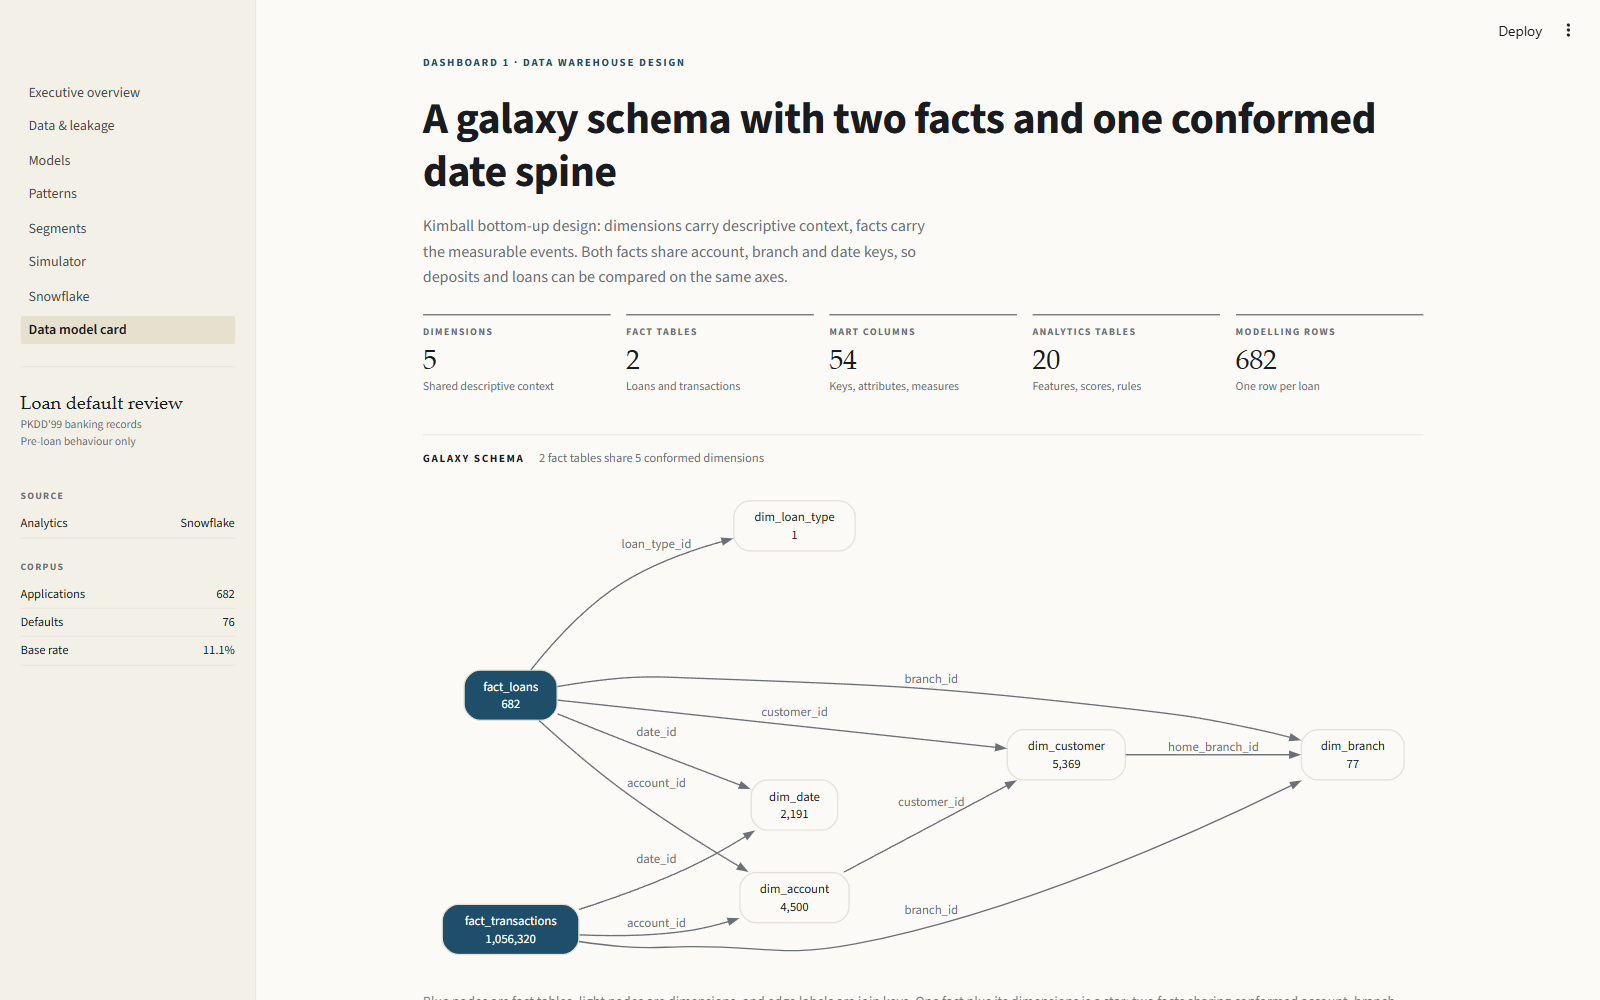
\includegraphics[width=0.92\textwidth]{figures/19_dashboard_data_model.png}
    \caption{Data model card page of the Streamlit dashboard}
    \label{fig:dashboard_datacard}
\end{figure}

The data model card is a Graphviz rendering of the galaxy schema, with an analytics row-count chart, the join keys between facts and dimensions, and a column dictionary. It is the fastest way for a jury to check that the warehouse design in Chapter~5 and the deployment in Chapter~4 describe the same objects.

\section{Jury Dashboard Map}
The jury guide asks for three dashboards mapped to rubric items. A single application supplies all three through separate pages, as shown in Table~\ref{tab:dashboard_map}.

\begin{table}[H]
    \centering
    \small
    \renewcommand{\arraystretch}{1.3}
    \begin{tabular}{|l|l|l|}
        \hline
        \textbf{Jury dashboard} & \textbf{Rubric item} & \textbf{App page} \\
        \hline
        Dashboard 1 & A $\cdot$ Data Warehouse Design & Data model card \\
        Dashboard 2 & B $\cdot$ Snowflake Deployment & Snowflake \\
        Dashboard 3 & C $\cdot$ Supervised Learning Dataset & Data and leakage \\
        \hline
    \end{tabular}
    \caption{Mapping of jury dashboards to Streamlit pages}
    \label{tab:dashboard_map}
\end{table}

The remaining rubric items are served by the other pages: classification by Models, pattern mining by Patterns, clustering by Segments, and the business recommendation by Executive overview and Simulator. Appendix~A gives the full rubric-to-evidence map.

\section{Supporting Figures}
Two static figures from the analysis are kept alongside the dashboard captures because they isolate results that the pages embed in larger layouts.

\begin{figure}[H]
    \centering
    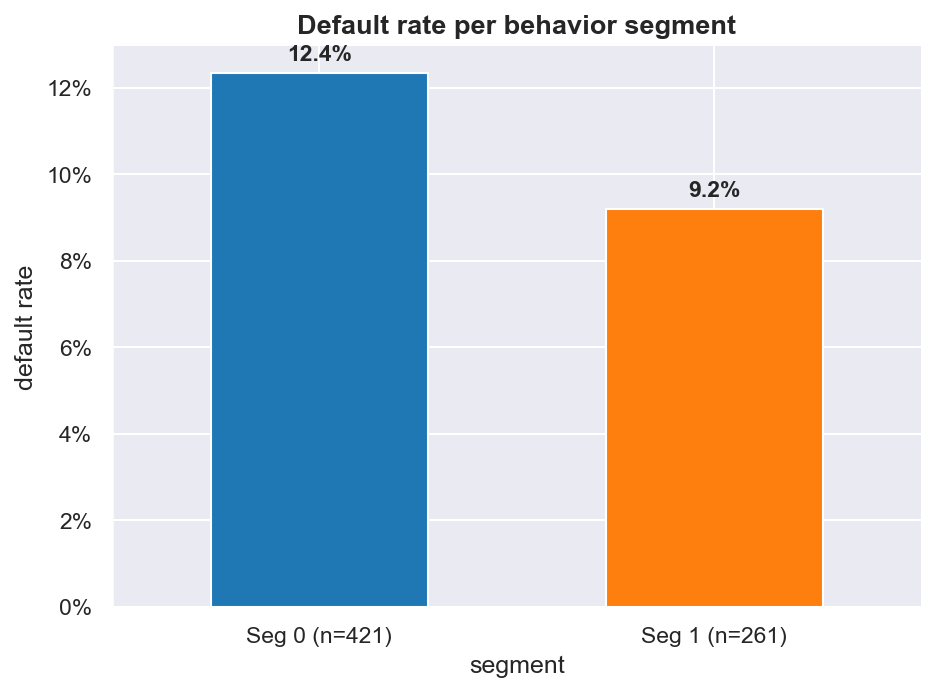
\includegraphics[width=0.88\textwidth]{figures/10_segment_default_rates.png}
    \caption{Observed default rate by behavioural segment}
    \label{fig:segment_rates_static}
\end{figure}

\begin{figure}[H]
    \centering
    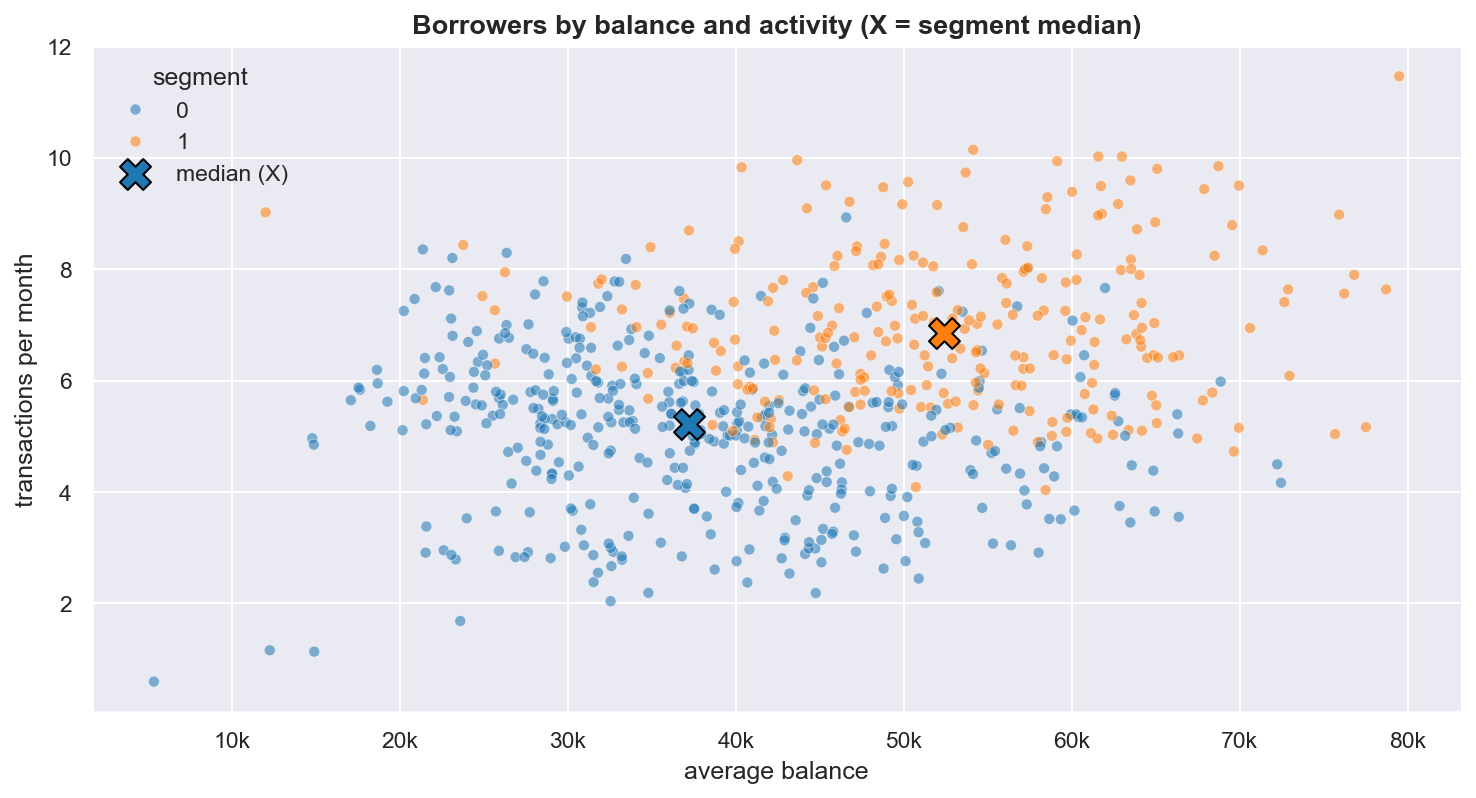
\includegraphics[width=0.88\textwidth]{figures/11_segment_scatter.png}
    \caption{Segment scatter used on the executive overview}
    \label{fig:segment_scatter_static}
\end{figure}

Together these views cover the full chain: warehouse structure, deployment evidence, leakage control, model comparison, mined rules, segments, and a single-loan score. Because every page is backed by saved artifacts rather than fresh computation, the figures in this chapter and the numbers in the earlier chapters are the same numbers.
